\chapter{Introduction}
\label{ch:chap1}


%------------------------------------------
\section{Backgrounds}

\subsection{Engineering Background}

In modern clinic room, the doctors are eagerly looking for a solution which can provide high fidelity and high resolution images to analyze the peripheral artery disease (PAD), which is a major cause of amputation in United States. PAD is prevalent among smokers, diabetics and patient with dyslipidemia. The  present technology can only render and deliver two-dimensional,  monochrome and static low-resolution picture. The long waiting time and high expense are two major problems for all the patients. In recent decades, researchers contribute numerous effort on improving the diagnosis of stenoses and the quality of imaging\cite{clark1976fluid, nesbitt2009shear, wardlaw2006non, stergiopulos1992computer, long2001numerical}. With the fast development on both hardware and numerical method, the computational simulation can provide 3-D, dynamic, high resolution and fast scan results. Comparing to current CT scan, it's more accurate, faster and cheaper. Moreover, it's also very important that the simulation strategy can bring the doctors and patients that the dynamic growth animations of current stenoses and the following consequence after the clinic treatment. Fig \ref{fig: ch1f1} summarizes some factors which contributing to the interests in computational medical simulation technology\cite{barry2005features}. Many investigations have been conducted through last decades\cite{feng2012viscous, bertram2010evaluation, nadeem2010simulation, ogulu2005simulation}. However, since this is a fluid-structural interaction (FSI) problem, both high fidelity fluid and solid solver are needed. 

\begin{figure}[H]
	\centering
	\begin{tabular}{c}
		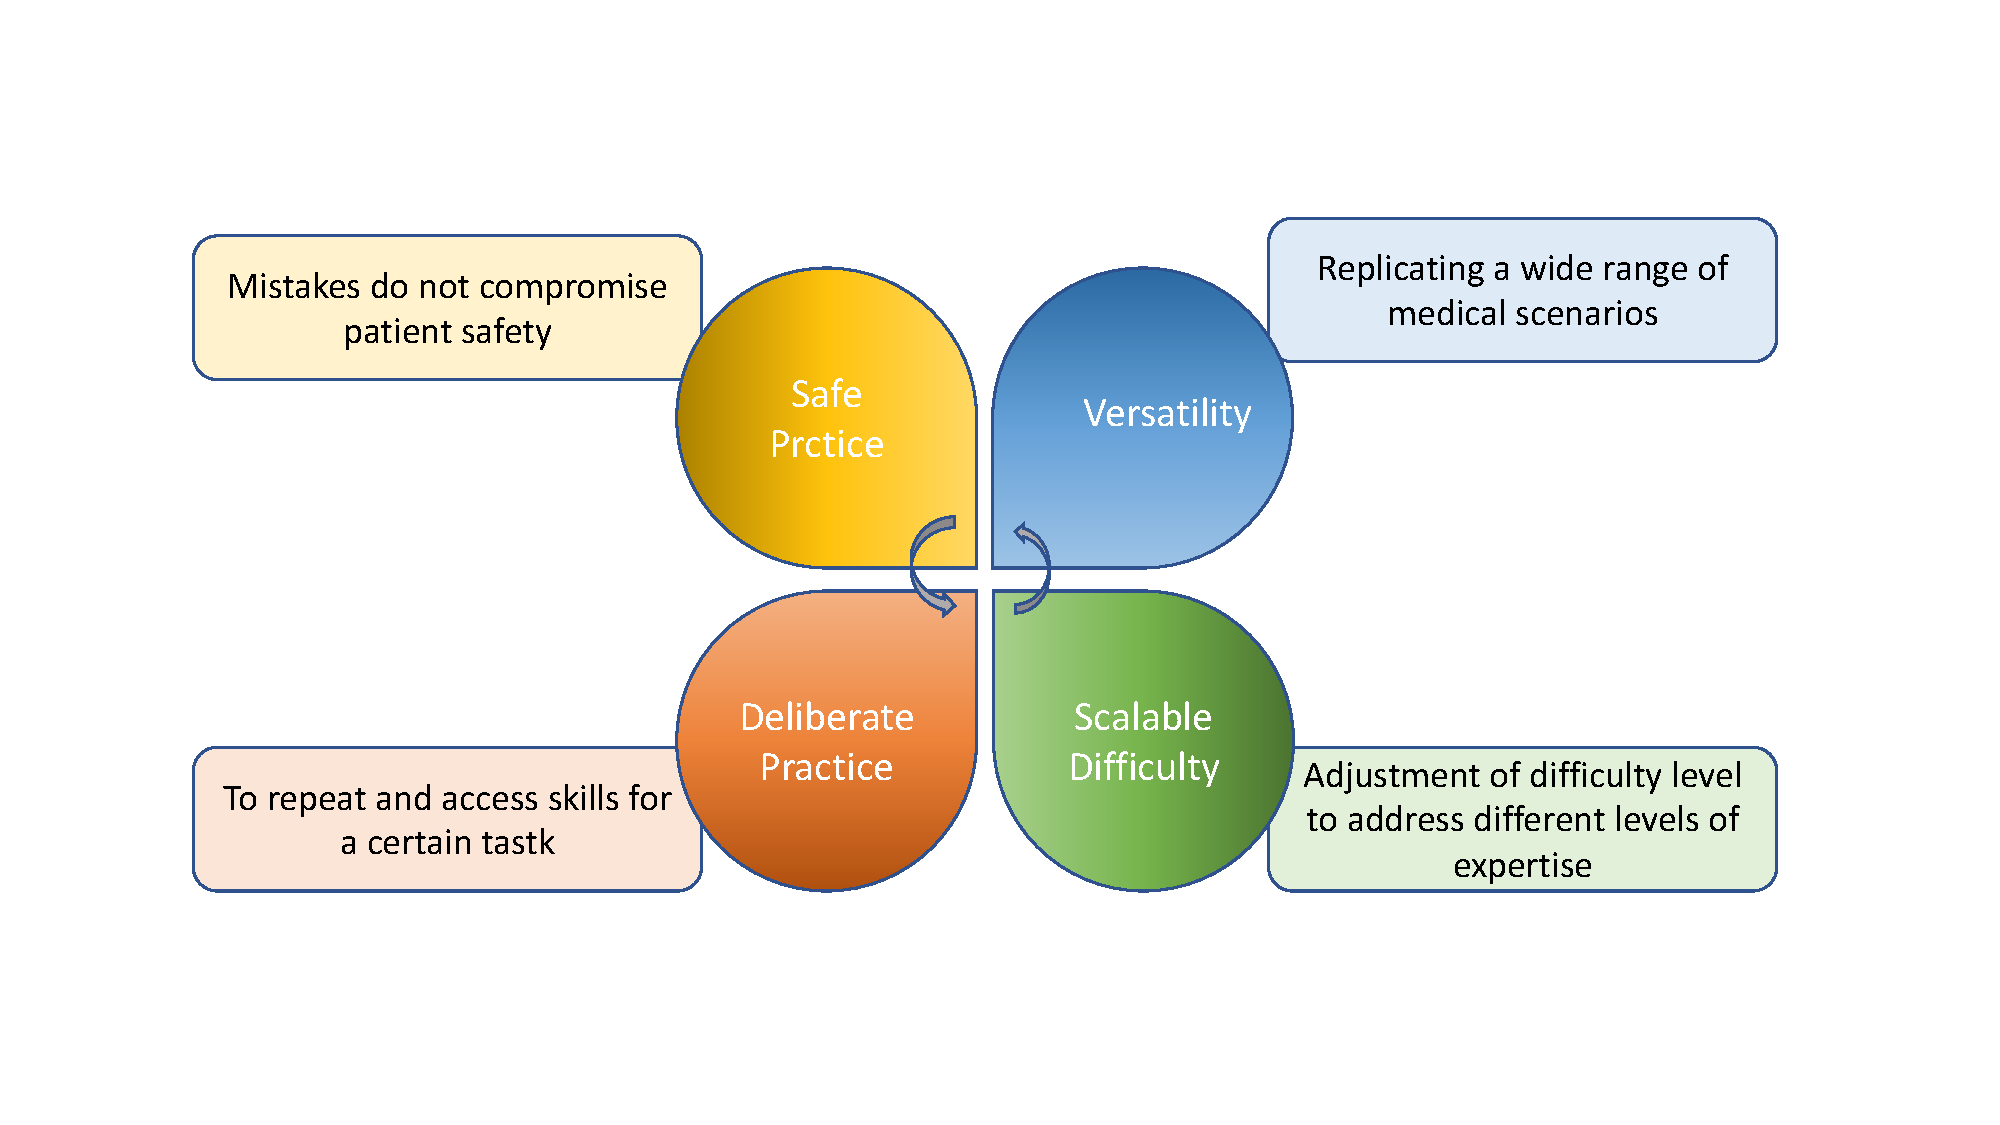
\includegraphics[width=1.0\textwidth]{./pics/computer_simulation}
	\end{tabular}
	\caption{\footnotesize Different factors affecting computer-based medical simulation.} \label{fig: ch1f1}
\end{figure}

The two most popular approaches for solving FSI problems are monolithic method and partitioned method. In the monolithic approach, the two sets of equations, fluid and structural, are solved simultaneously. The mutual influence of each other can be considered directly. The obvious advantage of this scheme is simplicity. Only one global matrix is needed so that both the fluid and structural parts can be solved within the same space discretization and time marching scheme. On the contrary, we lose the flexibility to precisely control each partition. The other approach is partitioned method. The two sets of equations are solved separately and pass boundary condition to each other like a cycle. The solution of fluid equations is calculated while the structural part is waiting for new input and vice versa. A coupling algorithm to exchange the interaction solution between two phases as a pair of modules. The Implicit-Explicit (IMEX) Runge-Kutta (RK) time integration approach has been proved the accuracy and efficiency on high order schemes\cite{zhang2016high}.

The high order parallel fluid solver \cite{liang2007large, liang2007large, liang2009effect} is accomplished and a series of CFD studies has been conducted along the ideal geometries. To implement the more realistic simulation, the tissue of blood vessel wall shall be considered as elastic material. An accurate and efficient solver for elasticity equation is needed. The solver should be capable on calculate the material behavior according to the stiffness property, which is the response of the deformable model reacting to the external forces. The simplest model is mass-spring model which is easy to compute but can not accurately determine the material behavior. The finite element method, which based on the continuum mechanics, has gained popularity since the results are more reliable. On the contrary to the mass-spring model, the FEM can specify the stiffness of the model by only using a few characteristic parameters, such as Young's modulus, Poisson ratio and geometries. However, the challenges for FEM is very difficult to be used in real-time application due to the very high computational expense. 

\begin{figure}[H]
	\centering
	\begin{tabular}{c}
		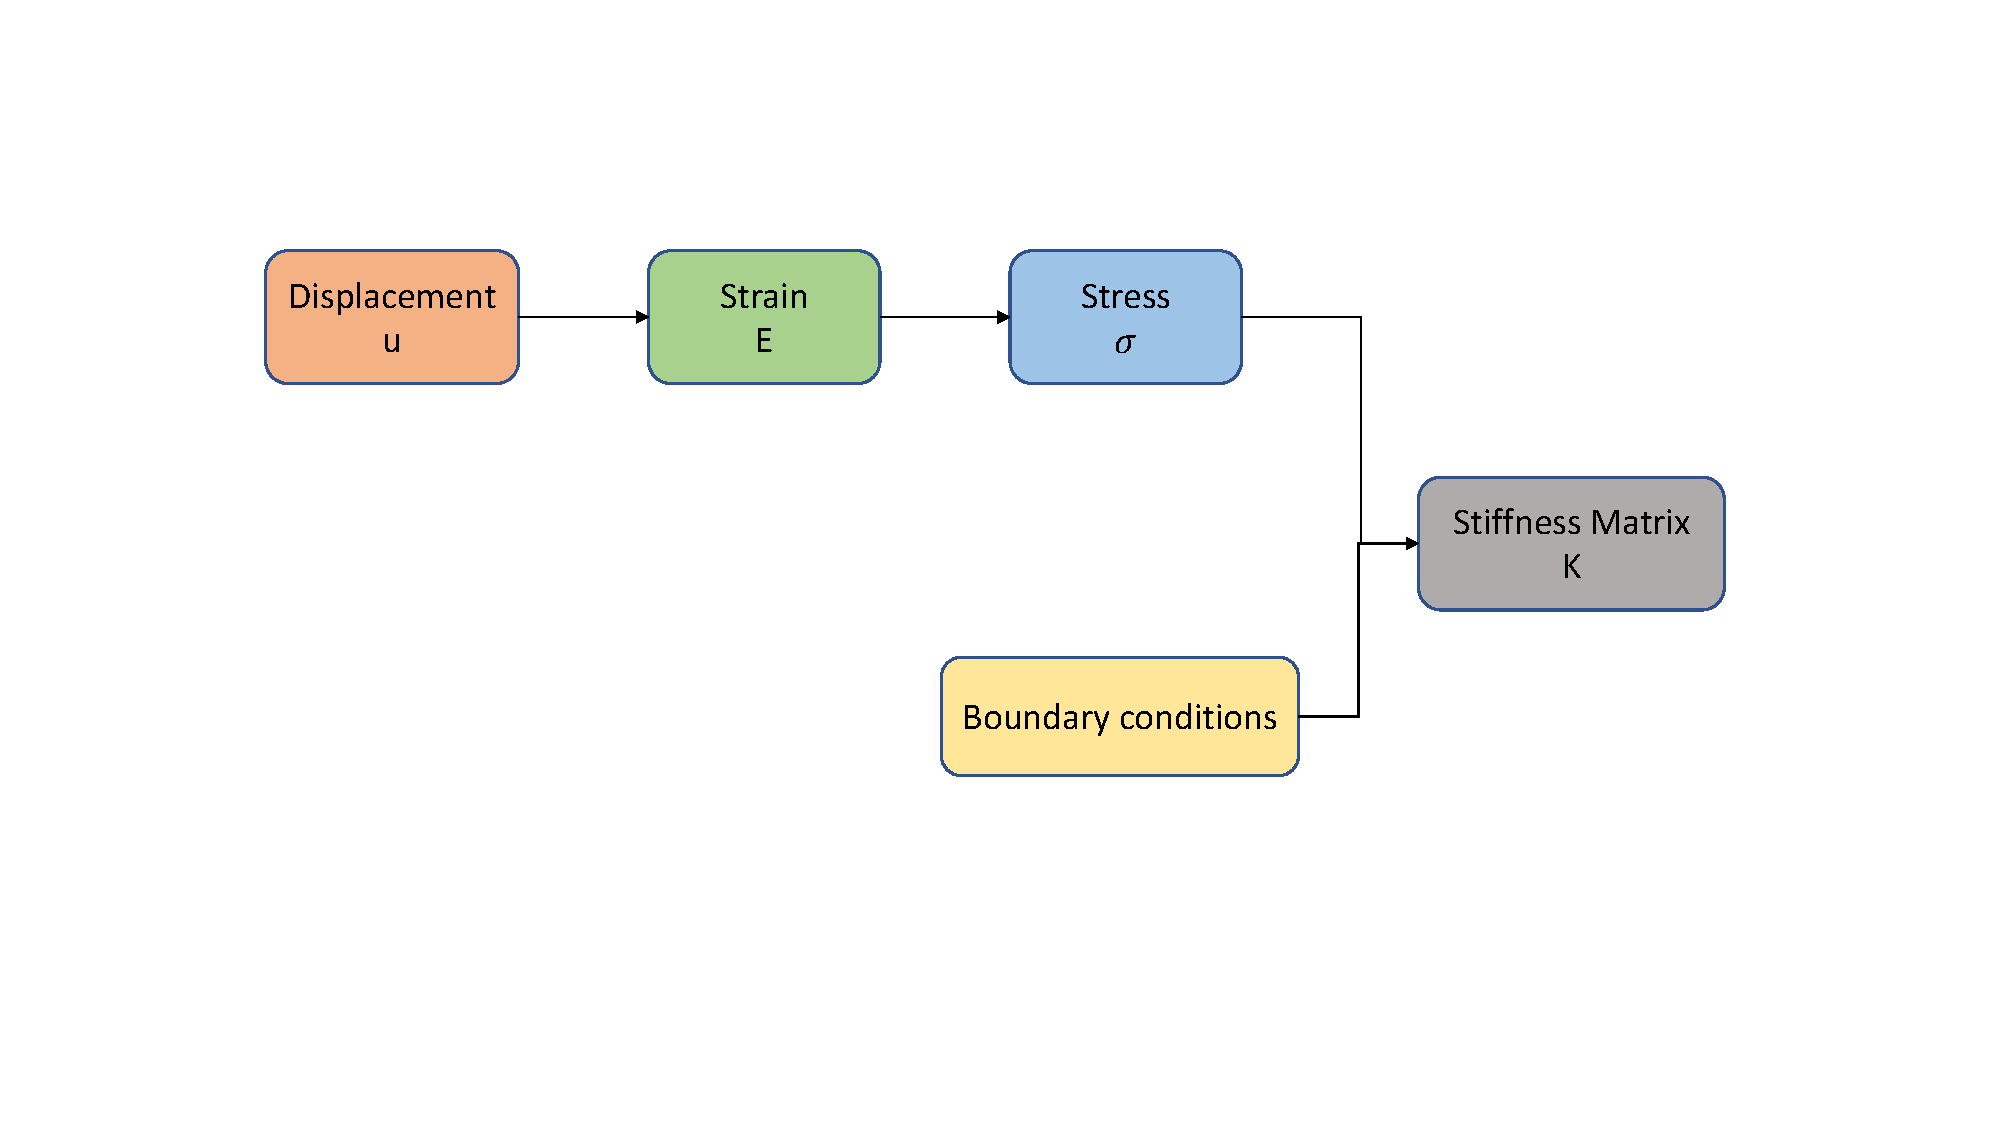
\includegraphics[width=1.0\textwidth]{./pics/construct_matrix}
	\end{tabular}
	\caption{\footnotesize Construct stiffness matrix.} \label{fig: ch1f2}
\end{figure}

Fig \ref{fig: ch1f2} shows a general process of calculating the stiffness matrix of a deformable material object. The stiffness matrix is derived from the gradient of stress which is calculated by the displacement and material property. The boundary conditions are imposed by the contact interaction.

\begin{figure}[H]
	\centering
	\begin{tabular}{c}
		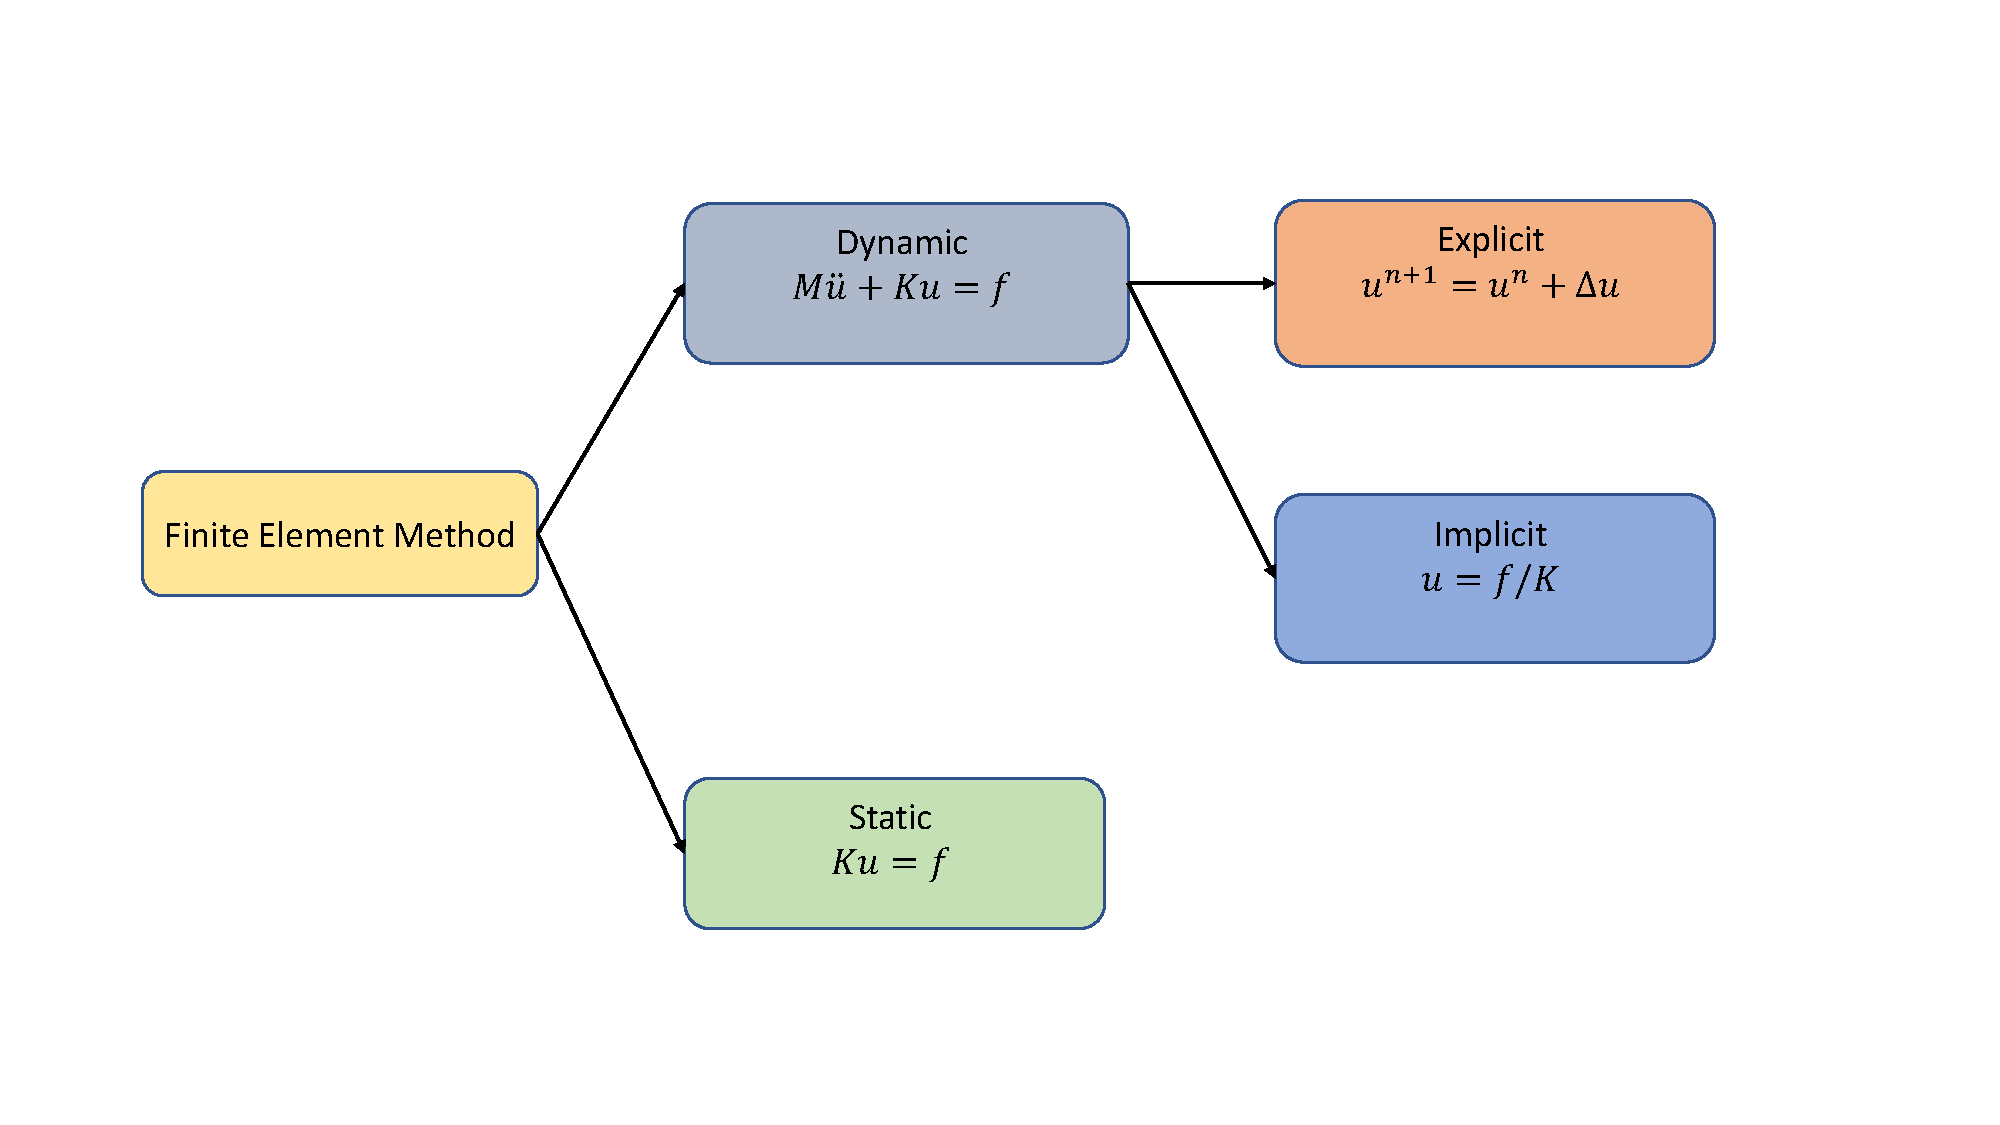
\includegraphics[width=1.0\textwidth]{./pics/fem}
	\end{tabular}
	\caption{\footnotesize Static and dynamic finite element method.} \label{fig: ch1f3}
\end{figure}

The Fig \ref{fig: ch1f3} displays both static analysis and dynamic analysis for a set of linear system of elasticity equations. The steady-state and transient finite element problem are studied with static analysis and dynamic analysis respectively. The latter is time dependent. In dynamic analysis, we shall consider the spatial discretization by using both explicit and implicit time integration schemes\cite{bathe2008finite}. The implicit time marching scheme is computationally costly, since the matrix inversion for linear system is required every time-step, similar to solving the static problem. The benefit is unconditionally stable for large time step. On the other hand, the explicit time marching scheme requires much lower computational cost as no linear solver is involved for each time-step. However, the size of each time step has to satisfy the numerical stability criteria. 


The linear system of elasticity equations derived from the FEM method is positive definite and too large to be direct inverse. The most time consuming part in the FEM analysis in Fig \ref{fig: ch1f2} is solving linear system. The complex system can be simplified as a matrix form $ \mathbf{A} \mathbf{x} = \mathbf{b} $. There are two main group of algorithms, direct and iterative method, to solve it. Considering the better performance on memory usage and computing time, the iterative method gains more affirmatives\cite{brussino1989comparison}. Preconditioned Conjugate Gradient (PCG) is the one of the best performance method because of its robustness and low computational cost. However, it is still very challenging to implement finite element analysis using implicit scheme to study the material real-time response behavior. The domain decomposition method combined with parallel computing scheme is one emerging choice to achieve that goal.

Parallel computing requires extra effort to tailor the algorithm to achieve concurrent execution. The challenges to reach that purpose include learning and understanding programming paradigms, design the balance load to maximize the usage of bandwidth, minimize the overhead on data communication and synchronization and avoid potential data race problems. The high performance computation based on CPU clusters is very challenging dealing with the complex hardware architecture and associated distributed memory. Some modern techniques such as MPI, Math-Kernel library and LAPACK-BLAS assist us to achieve optimal scalability. The key point for accomplish promising performance is to reduce the overhead latency by employing large number of active processors and ensure the balance of loads on each processor.

\subsection{Numerical Method Review}

The Weak Galerkin Finite Element Method (WG-FEM)is a novel developed, effective numerical method for solving partial differential equations. The WG method is first developed by Dr. Junping Wang and Xiu Ye in 2011, and applied on solving second order elliptic equation\cite{wang2014weak}. The main theory of WG method is to introduce a series of weak operators such as weak gradient, weak divergence and weak curl on the computation of corresponding forms of differential equations. The WG finite element method provides a  brand new perspective to solve numerical problems. It builds up the classic Continuous Galerkin(CG) method to an advanced stage. The WG method can be applied on variety of partial differential equations include second order elliptical equation, elasticity equation\cite{wang2016locking}, Stokes equations \cite{wang2016weak} and Maxwell's equations \cite{mu2013weak}, etc. The WG method inherits the discontinuity from the discontinuous basis functions. The construction of discrete matrix is independent with any external coefficients. The interior unknown variables can be eliminated to the boundary unknown variables to construct a linear system which only consists by degree of freedom(DOFs) along the element boundary. Even though the total DOF of WG method is larger than Discontinuous Galerkin method (DG), the interior unknown variables can eliminated through Schur complement method. The only left DOFs are along the element boundary which are far less than DOFs in DG finite element method. The elemental stiffness matrix of WG method can be constructed upon each element, which is consistent with CG FEM method. 

%-----------------------------------------------------
\section{Objectives of this Work}

The CG FEM analysis of continuum mechanics is widely used to study and predict the material deformation. The results are generally accurate and reliable in analyzing load and deformation. However, the computational complexity and cost inhibits the application on targeting the real-time FSI problems. Massive parallel computing is required for obtaining large linear system. In this work, we investigate methods for efficient parallel scheme which enables high-order novel finite element method in solving elasticity equation.

We employ the WG-FEM to convert the bilinear form equations into a positive definite linear system. The WG method has the capacity on varying high-order elements. The selection of polynomials on interior or boundary region is flexible which enhance the freedom on computational simulation. Moreover, the discontinuity features in the WG method which empower the parallel computation capability.

The Balancing Domain Decomposition by Constraints (BDDC) method is an ideal candidate for entitling the massive parallel capacity to WG-FEM. BDDC identifies the two spaces (primal and dual) to split the original computational domain. By minimizing the global communication and synchronization overhead,  WG-BDDC enriches the scalability of elasticity equations as a superlinear speedup curve.

The main objective of this thesis is to achieve fast, accuracy and scalability in WG-BDDC based analysis. Fig \ref{fig: ch1p4} shows the paths to accomplish the objectives in this work. The results of the research are significantly improving the computation of the elastic material response, including in clinic judgment and other medical applications.

\begin{figure}[H]
	\centering
	\begin{tabular}{c}
		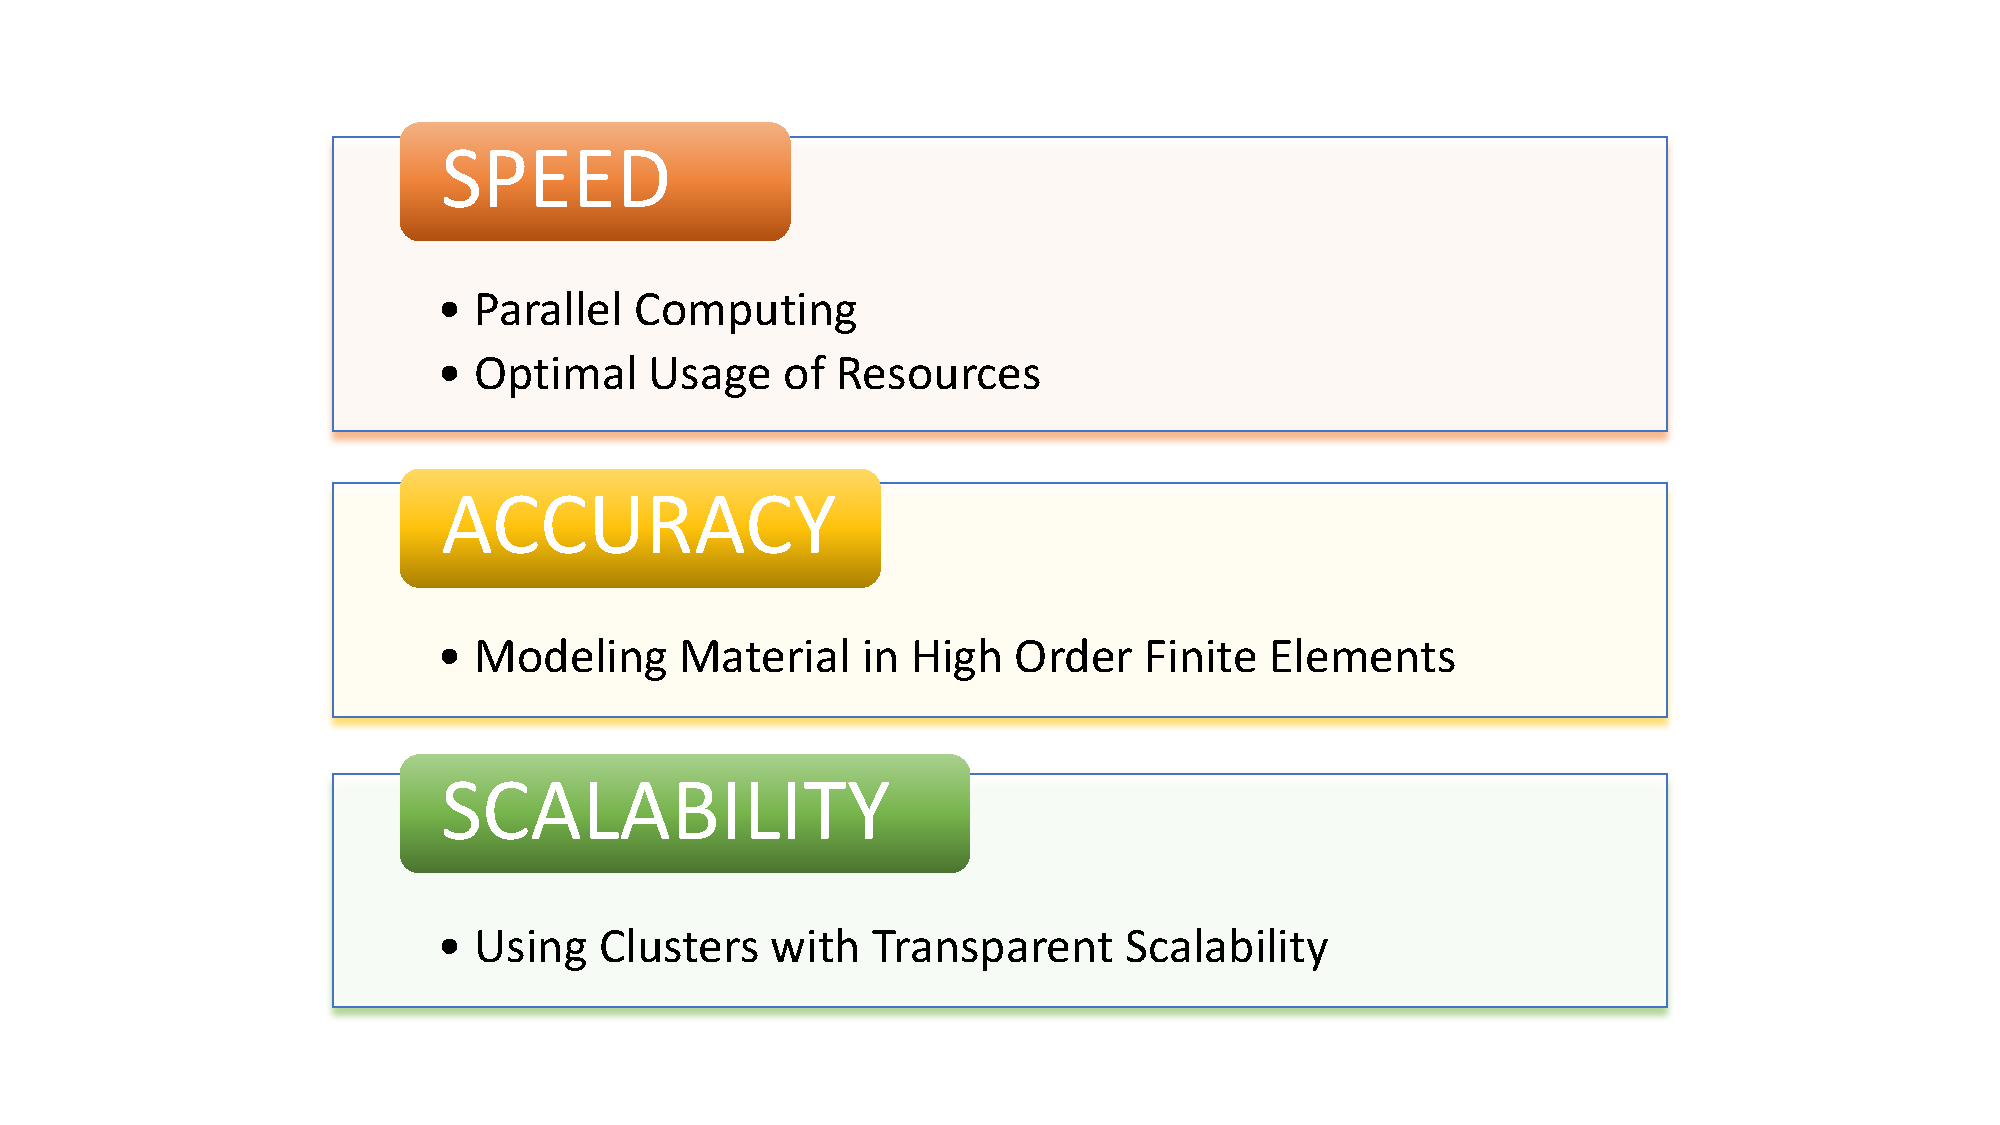
\includegraphics[width=1.0\textwidth]{./pics/ch1p4}
	\end{tabular}
	\caption{\footnotesize Objectives and methodology.} \label{fig: ch1p4}
\end{figure}

To validate the WG-BDDC scheme and develop the software, we first design the hybrid WG-CG element. The results are consistent with the benchmark of CG only element so the fidelity is proved. Then we extend the WG element to BDDC method and verify the properties of convergence and the order of accuracy with parallel fashion. Finally, the scalability is discussed under the parallel computing framework.

The rest of this dissertation is organized as :

\begin{itemize}
	\item Chapter 2 presents the background and basics of WG method.
	\item Chapter 3 discusses the hybrid WG-CG element the performance on nonlinear elasticity equation.
	\item Chapter 4 introduces the WG-BDDC method for second order elliptic and elasticity equation.
	\item Chapter 5 shows the study of effect multiple stenoses on the peripheral artery diseases.
	\item Chapter 6 concludes this work and outlook the future work.
\end{itemize}
